\section{Převodníky AD s vysokými vzorkovacími kmitočty}
- komparační, řetězové - základní zapojení a funkce, příklady využití.
\begin{figure}[h]
   \begin{center}
     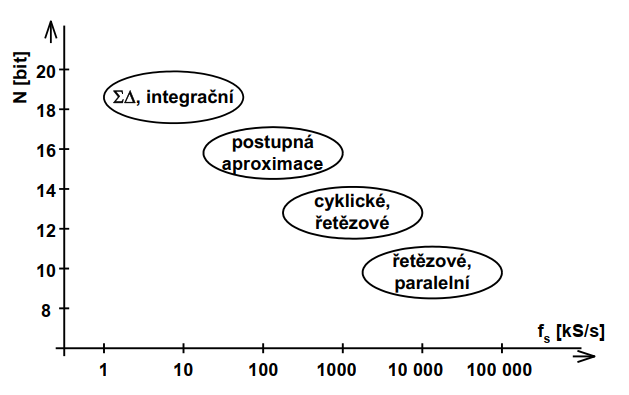
\includegraphics[scale=0.6]{images/ADroz.png}
   \end{center}
   \caption{Rozdělení ADC podle rozlišení v závislosti na četnosti převodu}
\end{figure}
\begin{figure}[h]
   \begin{center}
     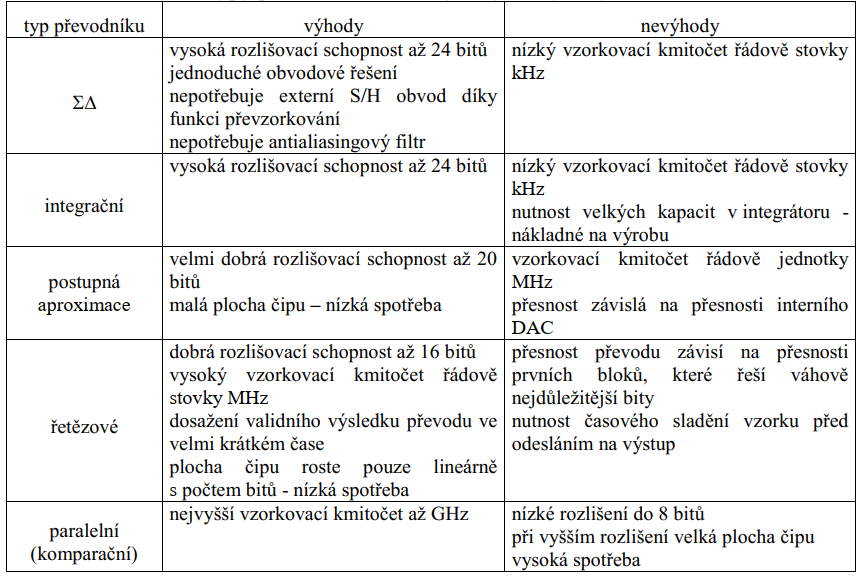
\includegraphics[scale=0.6]{images/ADroztab.png}
   \end{center}
   \caption{Základní typy převodníků AD – výhody, nevýhody}
\end{figure}
\subsection{Komparační}
Využívají přímou komparaci kvantovaného měřeného a referenčního napětí. Mohou dosáhnout extrémně krátké doby převodu. 

Nevýhodou je velký počet komparátorů a složitost dekodéru, uplatňující se u vícebitových převodníků. 

Kompenzační převodníky AD pracují na základě kompenzace měřeného napětí výstupním napětím řízeného převodníku DA. Z hlediska způsobu generace kompenzačního napětí lze rozlišovat ještě kompenzační převodníky s přírůstky kompenzačního napětí shodné a odstupňované velikosti. Integrační převodníky AD využívají řízené integrace měřeného a referenčního napětí, umožňují dosáhnout vysoké přesnosti převodu.

\textbf{Přímé převodníky AD} převádějí vstupní analogové napětí přímo na výstupní slovo. 

U \textbf{nepřímých převodníků AD} je vstupní analogové napětí převedeno nejprve na jinou analogovou veličinu (např. čas, kmitočet) a teprve potom je tato pomocná analogová veličina převedena do číslicového tvaru.
\begin{figure}[h]
   \begin{center}
     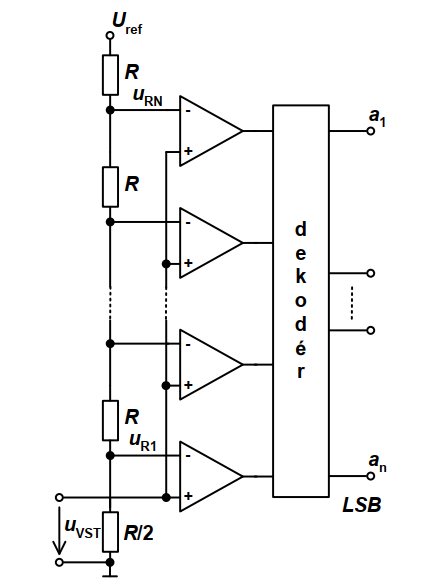
\includegraphics[scale=0.6]{images/ADkomp.png}
   \end{center}
   \caption{Zapojení paralelního komparačního převodníku AD}
\end{figure}

U paralelního typu je vstupní signál přiveden paralelně na řadu komparátorů. Na každý komparátor je rovněž připojena poměrná část referenčního napětí získaná na rezistorovém děliči zhotoveném z řady shodných rezistorů s odpory R. Pro každou možnou kvantovací hladinu existuje příslušná napěťová komparační úroveň. Komparační úrovně jsou v souladu s převodní charakteristikou  voleny do středu intervalů mezi jednotky vstupního napětí. Proto se například napětí u$\in$(2,5; 3,5 V) vyhodnotí aritmeticky správně, u = 3 V. Posun o polovinu kvantovacího bloku je docílen spodním rezistorem s odporem R/2 v rezistorové síti převodníku.

Přivede-li se libovolné dovolené vstupní napětí, všechny komparátory srovnávají jeho hodnotu s kvantovacími hladinami. Tyto komparátory, jejichž referenční úroveň je menší než vstupní napětí, nastaví na svém výstupu úroveň 1, u ostatních komparátorů bude na jejich výstupech logická nula. Výstupy všech komparátorů jsou vedeny na dekodér, kde se získá paralelní výstupní kód.

Tento ADC je
extrémně rychlý. Jeho rychlost je prakticky limitována jen rekreační dobou komparátorů
a dekódovací logiky. Jeho složitost však exponenciálně roste s počtem bitů.

\subsection{Řetězové}
V zájmu zmenšení počtu komparátorů a dodržení velké rychlosti převodu byly vyvinuty řetězové převodníky AD.

Typický řetězový ADC se skládá z několika stejných bloků (stupňů), které jsou kaskádně propojeny za sebou. Každý stupeň převodníku se skládá ze vstupního vzorkovacího obvodu, subADC a subDAC. Princip funkce je pro všechny stupně stejný. Vstupní signál je kvantován, pomocí subADC převeden do binární podoby a jako částečný výstup je poslán do bloku korekce. Mezitím je však opět pomocí subDAC převeden zpět do analogové podoby a odečten od původního vstupního signálu. Výsledné residuum u\textsubscript{res}, je pak ještě zesíleno a odesláno do dalšího stupně. První bloky tedy řeší nejvýznamnější bity (MSB) převodu, naopak nejméně významné bity řeší poslední blok, kterým je většinou jen několikabitový paralelní převodník.
\begin{figure}[h]
   \begin{center}
     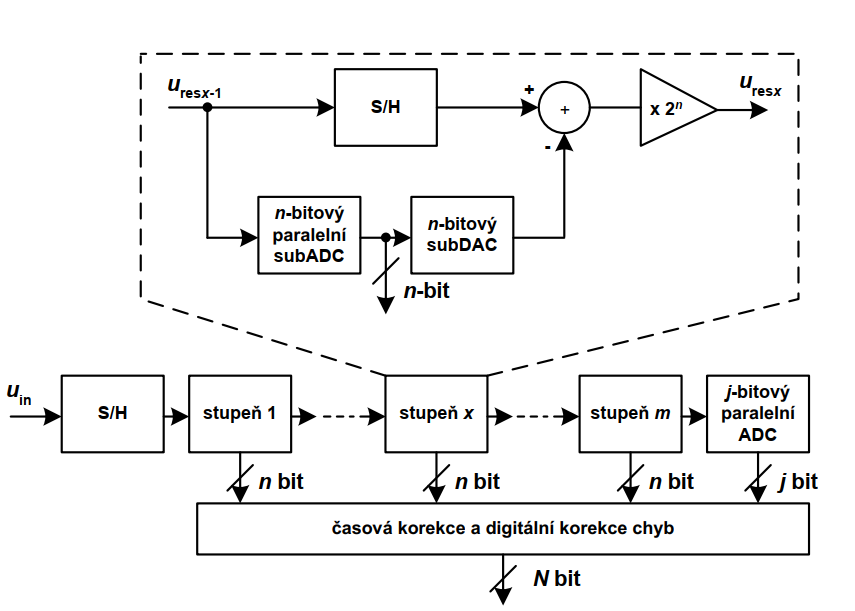
\includegraphics[scale=0.6]{images/ADret.png}
   \end{center}
   \caption{Princip řetězového ADC}
\end{figure}

\pagebreak
MDAC má rozlišení 1,5 bitu, což je nejčastěji používané rozlišení, a to
z několika důvodů. Při tomto rozlišení je dosaženo maximální šířky pásma a při zesílení 2
uzavřené smyčky je malá kapacitní zátěž a velký faktor zpětné vazby. Při tomto rozlišení
nedochází ani k degradaci celkové linearity převodu a SNR v důsledku nesymetrie
komparátoru. Navíc čím vyšší je rozlišení na stupeň, tím větší je i spotřeba obvodu.
\begin{figure}[h]
   \begin{center}
     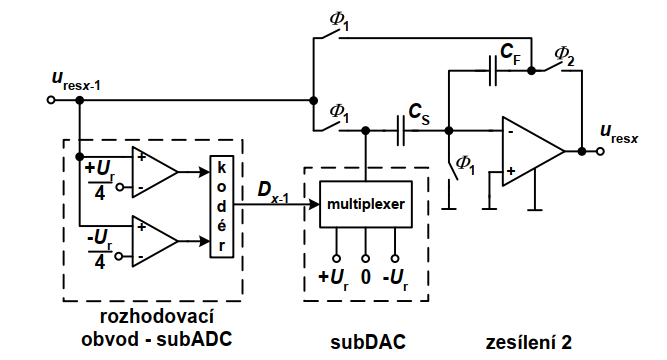
\includegraphics[scale=0.6]{images/MADC.png}
   \end{center}
   \caption{MDAC realizovaný technikou SC}
\end{figure}
\begin{figure}[h]
   \begin{center}
     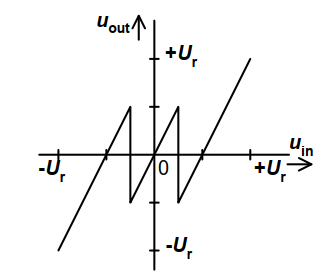
\includegraphics[scale=0.6]{images/MADCprev.png}
   \end{center}
   \caption{Převodní charakteristika 1,5-bitového MDAC}
\end{figure}

\pagebreak
\textbf{Použití:} v bateriově napájených zařízeních, dále v medicíně, komunikačních modulech apod.




